\section{Introduction}

This manual gives an overview on the Elmer software package. The emphasis is on the total view
and the user is encouraged to read the other Elmer manuals for more detailed information. 

\subsection*{What is Elmer}

Elmer is a finite element software package for the solution of partial differential 
equations. Elmer can deal a large number of different equations which may be coupled 
in a generic manner making Elmer a versatile tool for multiphysical simulations. 


\subsection*{History of Elmer}
The development of Elmer was started in 1995 as part of a national CFD technology 
program funded by the Finnish funding agency for technology and innovation, Tekes. 
The original development consortia included partners from CSC - The Finnish IT Center 
for Science, Helsinki University of Technology TKK, VTT Technical Research Centre of Finland,
University of Jyv�skyl�, and Okmetic Ltd. After the five years initial project ended 
the development has been continued by CSC in different application fields.

\subsection*{Licensing}
In September 2005 Elmer was released under GNU General Public Licence (GPL). This 
has meant a significant growth particularly of the international user community. 
However, as the sole owner of the copyright to Elmer source code CSC may distribute 
Elmer also under other licensing terms. Therefore if GPL does not suit your purposes 
you may contact the Elmer team for other licensing options. 

\subsection*{Distribution}
Elmer is distributed only through the Internet. The actual distribution place may vary 
but the pointer to the distribution may always be found at \URL{http://www.csc.fi/elmer}. 

The distribution of Elmer comes in three different parts: sources, binaries and documentation.
In Unix systems the users are encouraged to 
compile the software themselves. The current compilation instructions are given at the www-page.
For Windows and Macintosh a precompiled binary version of the code is provided. 
The documentation is already quite large, but unfortunately still not complete.


\section{Key features of Elmer}

Elmer includes a huge number of capabilities in different categories. This list summarizes 
some of the most essential ones.

\subsection*{Physical models in Elmer}
\begin{itemize}
  \item Heat transfer: conduction, radiation and phase change
  \item Fluid flow: Navier-Stokes, Stokes and Reynolds equations, k-$\varepsilon$ model
  \item Species transport: generic convection-diffusion equation
  \item Elasticisty: Generic elasticity, plates, shells
  \item Acoustics: Helmholtz equation
  \item Electromagnetics: electrostatics, magnetostatics, induction
  \item Microfluidics: slip conditions, Poisson-Boltzmann
  \item Levelset method: Eulerian free boundary problems 
  \item Quantum Mechanics: Density functional theory (Kohn-Sham)
\end{itemize}

\subsection*{Numerical methods in Elmer}
\begin{itemize}
  \item All basic Langrangian elementtypes in 1D, 2D and 3D in 1st and 2nd degree
  \item Generic p-base elements
  \item Discontinous Galerkin
  \item Stabilization with residual free bubbles or with SUPG
  \item Adaptivity particularly in 2D 
  \item Iterative Krylov subspace solvers
  \item Direct solvers (Lapack \& Umfpack)
  \item Multigrid solvers (GMG and AMG) for simple problem types
  \item ILU Preconditioning 
  \item Parallelization of iterative methods
  \item BEM solvers (without multipole acceleration)
\end{itemize}

\subsection*{Pros and Cons of Elmer}
For potential users it may be useful to summarize some of the possible pros and cons 
or Elmer package. The list is naturally very subjective and not complete either.
\begin{itemize}
\item[+] Elmer is Open Source, therefore it is possible to verify and modify the solution procedures
\item[+] Elmer has an abstract treatment of physical equations making it is easy to adapt new fields
\item[+] All material parameters may depend on field variables and other parameters in a free manner
\item[+] Elmer offers a large selection of modern numerical methods
\item[+] Elmer enables most generally used element types 
\item[+] Elmer has a graphical preprocessing interface for simple problem setups
\item[+] Elmer has a steadily growing user community and it has been used in tens of scientific papers 
\item[+] Assembly and iterative solution is available also in parallel
\item[+] Elmer is easily compiled for most Unix systems and it is also available
  for Windows and Macintosh machines as precompiled binaries
\item[-] The graphical preprocessing interface to Elmer cannot utilize all the features of Elmer
\item[-] Getting to know the large package may take time. Previous experience on FEM packages 
  may therefore be useful
\item[-] Elmer does not include proper geometry or mesh generation tools for complicated problems. Only 
  mesh import interfaces are supported 
\item[-] As a multiphysical tool Elmer does not include all the physical details of the individual fields.
         For example, in turbulence and multiphase modeling Elmer has quite little to offer
\item[-] The documentation of Elmer is not always up-to-date
\end{itemize}





\section{Elmer executables}

As most finite element packages Elmer is divided into a number of different
executables that may also be used separately. The main packages are the preprocossor, solver
and postprocessor, but there also other modules that may called for specific assignments. 

\sifbegin
\sifitem{ElmerSolver}{}
ElmerSolver is the soul of the Elmer software and the part where most development work is 
directed to. ElmerSolver includes a large number of finite element library tools
which enable new equations to be written economically. The equations are mainly 
available as dynamical libraries with standard interfaces that are linked to the main 
program on request. 

\sifitem{ElmerPost}{}
ElmerPost is a versatile postprocessor that usually is quite sufficient for the postrprocessing
needs. ElmerPost provides a straight-forward graphical user interface that is easy to learn. ElmerPost
utilizes Mesa and TCL/TK graphics libraries. 

\sifitem{ElmerFront}{}
ElmerFront is the graphical user interface for setting up a simulation problem. 
ElmerFront is not actively developed and therefore a large part of the functionality of ElmerSolver
is not supported through ElmerFront. The meshing capabilities of ElmerFront are limited to 
2D Delaynay type of meshes which are obtained by calling the \texttt{Mesh2D} program. 
%Otherwise an existing mesh should be provided for the system. 

\sifitem{ElmerGrid}{}
ElmerGrid provides simple structured mesh generation functionality and may also be used 
for many kinds of mesh manipulation and transformation tasks. For example, ElmerGrid may be used
to partition the mesh for parallel runs or to import meshes written by other mesh generators. 
The ElmerGrid command file is to be written by a text editor. 

\sifitem{Mesh2D}{}
This is a Delaunay triangulator that is called by ElmerFront but may also be called independently
from command line.

\sifitem{ViewFactors}{}
This is a program for the computation of view factors that need to be determined in some radiation 
problems. Usually there is no need to call this separately as it is automatically called 
from within ElmerSolver.
\sifend



\section{Elmer modules}
The Elmer is distributed as partially interdependent modules. Some of them include binaries while
other are used as libraries only. Below is a possible distribution list. The first version number is changed in
major new releases while the second number indicates minor changes taking place few times in a year. 
Basically the user does not need to be aware of the module interdependencies unless she or he wants to 
setup only a partial system.

\sifbegin
\sifitem{eio-5.3.0.tar.gz}{}
Elmer input/output library written in C++. Used for some I/O operations by the ElmerSolver. 
\sifitem{elmergrid-5.3.1.tar.gz}{}	
ElmerGrid source codes written in C. Also includes the Metis library from the Karypis Lab. 
\sifitem{elmerpost-5.3.0.tar.gz}{} 	
ElmerPost source codes written in C. 
\sifitem{fem-5.3.0.tar.gz}{}	
ElmerSolver source codes written mainly in Fortran90.
\sifitem{front-5.2.0.tar.gz}{}
ElmerFront source codes written in C++.
\sifitem{hutiter-5.3.0.tar.gz}{} 
The iterative linear algebra solvers called by ElmerSolver. Written mainly in Fortran90.
\sifitem{matc-5.3.0.tar.gz}{} 
The library is used in the command file interpreter of ElmerSolver and inside the command 
window of ElmerPost for evaluating mathematical expressions written in C.  
\sifitem{mathlibs-1.0.0.tar.gz }{}	
Includes basic mathematical libraries such as Lapack, Blas, Arpack, and Parpack.
\sifitem{meshgen2d-5.0.0.tar.gz}{} 
Includes the source code of the 2D Delaynay mesher. 
\sifitem{umfpack-4.4.tar.gz}{}
Includes the source code of the Umfpack library from University of California.
\sifend


\section{Elmer file formats}
Elmer uses and creates variable number of files in the solution of the case. 
Here is some information about the Elmer file system. 

\sifbegin
\sifitem{ElmerSolver command file}{*.sif}
The command file that is read by the ElmerSolver in start of the simulation. 
The command file may be automatically written by ElmerFront, or it may be
edited by a text editor using appropriate example files as starting points.  
The Solver manual and Models manual provide the best source of information 
on the different keywords. 

\sifitem{ElmerSolver mesh format}{meshdir/mesh.*}
The mesh is defined by four different files \texttt{mesh.nodes},~\texttt{mesh.elements},
~\texttt{mesh.boundary}, and \texttt{mesh.header},
which are located in the mesh directory. The mesh may be created by 
Mesh2D directly or through ElmerFront, ElmerGrid, or by enhanced versions of 
Netgen and GiD. The file format is compatible with ElmerSolver, ElmerFront and ElmerGrid.

\sifitem{ElmerSolver result file}{*.result}
The result file of the simulation in a form that may be used to make a restart from a previous
set of results. ElmerSolver by default writes this file to the mesh directory. The file is 
compatible only with ElmerSolver.

\sifitem{ElmerPost file}{*.ep}
This file is written by ElmerSolver and can be read by ElmerPost. 
ElmerSolver by default writes this file to the mesh directory.
The file is used mainly for visualization purposes.

\sifitem{Elmer geometry format}{*.egf}
This format defines a 2D geometry using primitives such as points and lines. 
The geometry format is defined using an editor and it is 
read by the ElmerFront program. 

\sifitem{Elmer mesh input format}{*.mif}
This is the format that Mesh2D uses to create Delaynay triangulations. 
It is usually written by ElmerFront but it may easily be modified by an editor.

\sifitem{ElmerGrid mesh definition file}{*.grd}
This file is used to define 1D, 2D or 3D structured meshes. 
The file can only be read by ElmerGrid.

\sifitem{ElmerGrid command file}{*.eg}
This file is used to make mesh manipulation operations. The same functionality 
may be achieved by command line arguments.

\sifitem{ELMERSOLVER\_STARTINFO}{} 
This file is used my ElmerSolver and simply includes the name of the command file.
The other possibility to transfer the command file name to ElmerSolver is to use 
a command line parameter.

\sifitem{SOLVER.KEYWORDS}{}
The keywords of ElmerSolver are listed in a file located in the directory of the shared 
library files of ElmerSolver. This list is not complete as new keywords 
are always popping up due to the development work. Therefore the user may create a local file and 
add there the missing keywords. Note that it does not really matter if keywords are not defined,
as long as the type is given and in the command file the \texttt{check keywords warn} is used 
instead of \texttt{abort}. 

\sifend



\section{Elmer documentation}

The Elmer documentation is constantly under development. The version date of the manuals is 
printed in the cover of the manuals. The current set of Elmer manuals is as follows

\sifbegin
\sifitem{ElmerSolverManual.pdf}{}
	ElmerSolver Manual gives on overview of the capabilities of the solver with an 
	emphasis on generic services provided by the solver. This does not include information of 
	certain physical equations.
\sifitem{ElmerModelsManual.pdf}{}
	The Models Manual describes the different physical models that are defined
	in independent subroutines. This is quite well up-to-date. 
\sifitem{ElmerTutorials.pdf}{}
	The tutorials of the Elmer software are basically just example files with documentation.
	The relatex \texttt{ElmerTutorialFiles.tar.gz}
	provide the files related to the tutorials in a directory tree.
\sifitem{ElmerGridManual.pdf}{}
	The Manual of ElmerGrid utility.
	Examples related to the ElmerGrid documentation are provided in file 
	ElmerGridExamples.tar.gz.
\sifitem{ElmerFrontUserGuide.pdf}{}
	Manual for the graphical user interface ElmerFront. ElmerFront is not actively developed 
	and this might be the final documentation of the program.
\sifend
In addition to these manuals there are separate documentation for some input interfaces (GiD) and
for vizualization tasks (making animations). Look at the www-pages for more information on these
documents. 

Some useful information may also be found in the following old documents.
\sifbegin
\sifitem{OldElmerUserGuide.pdf}{}
	The original user guide of Elmer software (1999). Particularly some appendixes defining some of the 
	file formats may still be useful.
\sifitem{OldElmerTutorial.pdf}{}
	A graphical user guide oriented tutorial of the Elmer software (2000). 
\sifend

\begin{figure}[tbhp]
\vspace{-20mm}
\begin{center}
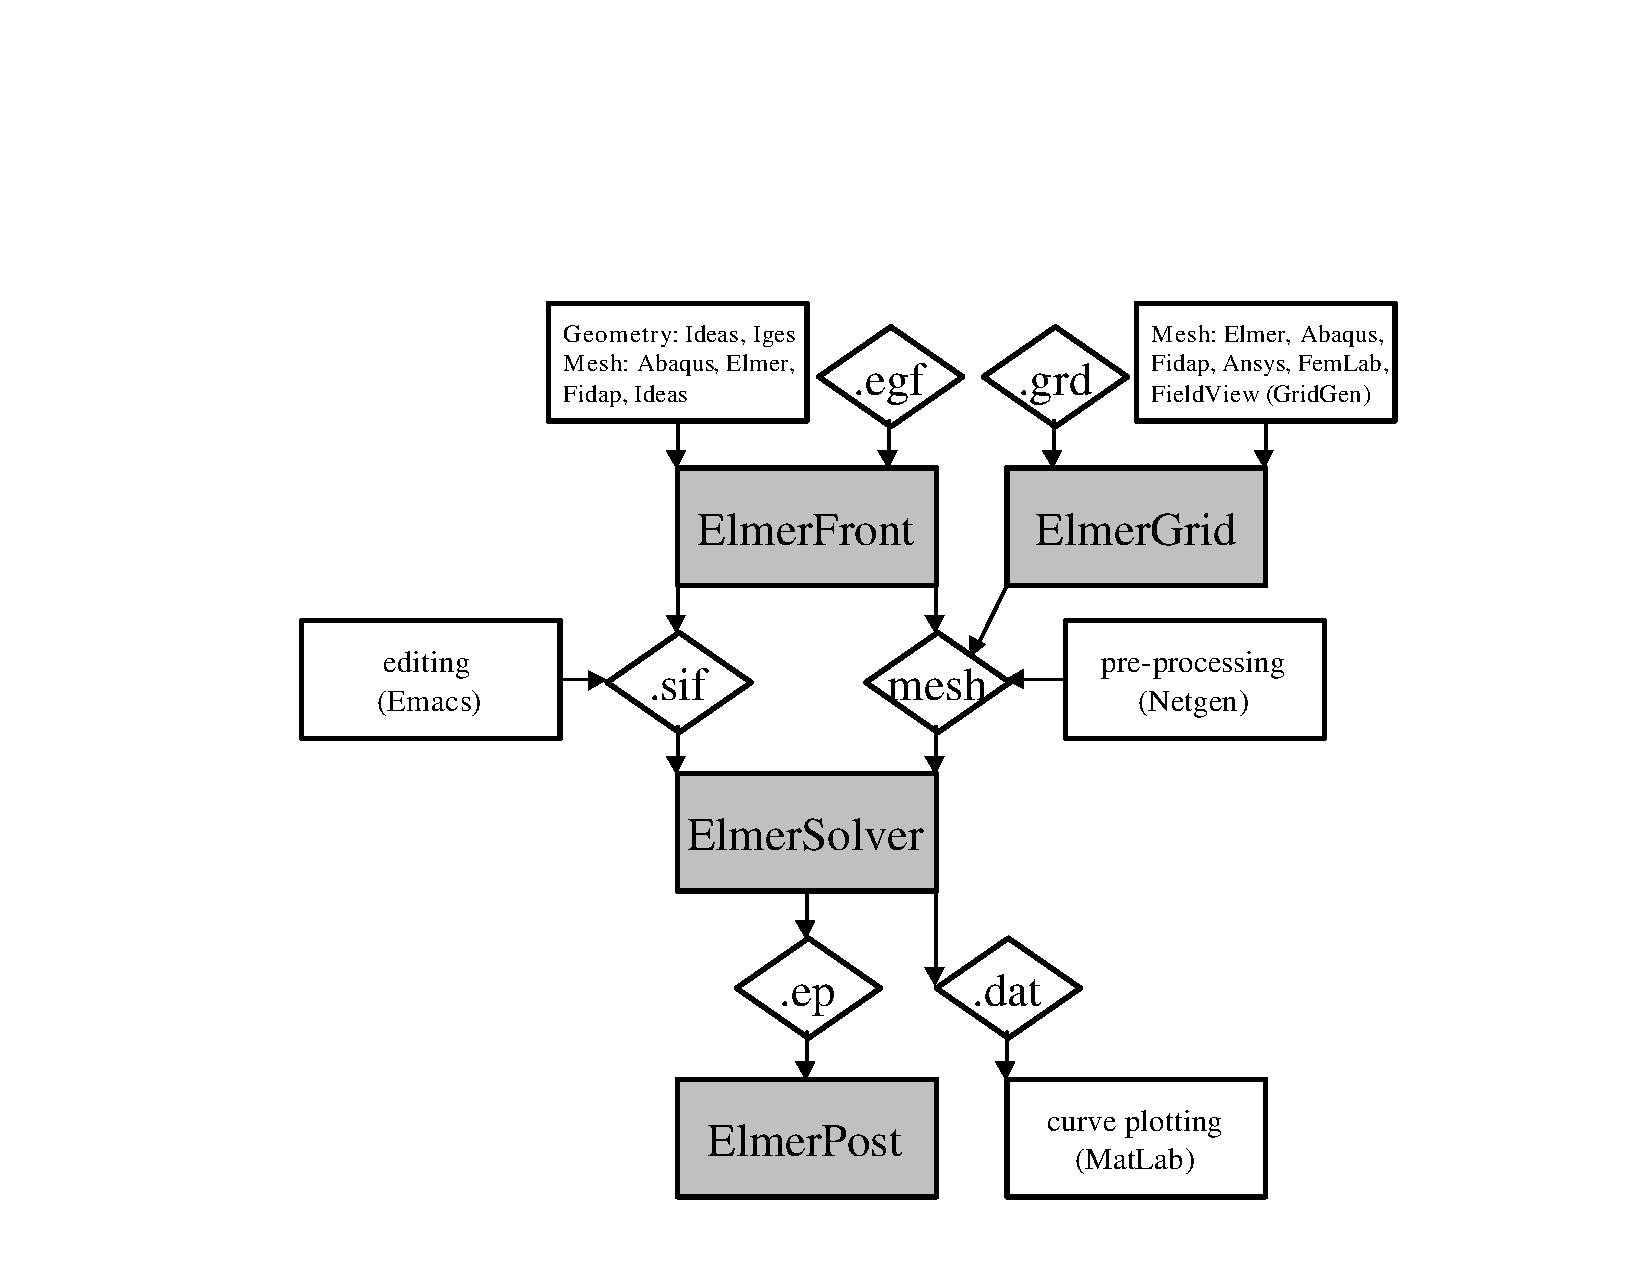
\includegraphics[width=13.0cm]{elmer-chart.pdf}
\caption{Work flow in the Elmer environment}
\label{fig_workflow}
\end{center}
\end{figure}



\section{Strategies for using the Elmer package}

Because of the number of different modules in Elmer there is a number of different strategies
how use Elmer. 
Here we try to explain the different choices in more detail. 
Examples on the different choices strategies may be found in Elmer tutorials. 
Figure~\ref{fig_workflow} shows a schematic pictures on how the different components depend
on one-another.



\subsection*{Strategies for preprocessing}

The purpose of the preprocessing phase is to create the ElmerSolver input files, which 
are at the minimum the command file and the mesh files. 


\subsubsection*{Geometry definition + ElmerFront}

The simplest way to create a simulation from scratch is to use an existing 
geometry definition (egf or 2D CAD file) and ElmerFront. 
A handicap with ElmerFront is that it does not have any geometry definition tools,
and the mesh generation tools are limited to 2D Delaynay. 
ElmerFront is then used 
to define the equations, boundary and initial conditions, and material parameters. 
For the solution ElmerFront calls ElmerSolver automatically, and likewise ElmerPost for the visualization. 

A large partion of the capabilities of ElmerSolver are not supported in ElmerFront. 
Therefore ElmerFront as the only strategy is best suited for relatively simple tasks with the standard equations
(heat, flow, stress). The good thing is that the user does not need to get acquinted with the 
different file formats, nor edit them by hand. Also the user does not need to restart any other 
binary except ElmerFront. Serious users have to abandon this as the 
only strategy quite soon. 


\subsubsection*{Your favorite mesh generator + ElmerFront}
Besides of its own meshing capabilities ElmerFront can read  
an existing 2D or 3D mesh. The supported formats include Abaqus, 
Fidap neutral file, Ideas universal file and Elmer mesh format. 

\subsubsection*{Editing command files created by ElmerFront}


ElmerFront may be used as a first step in the simulations, even though that in most of cases it 
cannot be used for full setup of the case. Making a preliminary command file and/or mesh with 
ElmerFront often saves some time. Thereafter this command file (*.sif) may be modified by some
text editor (e.g. emacs) to account for more detailed specification. In adding the keywords in the
command file, the Models Manual is of greate help. The ElmerSolver and ElmerPost 
are in this approach executed by the command line. 



\subsubsection*{ElmerGrid + editor}

An easy way to make simple 2D and 3D meshes is to use ElmerGrid. The mesh definition file 
of ElmerGrid also defines the geometry. However, the structured format of ElmerGrid favors
box like forms and making more complicated shapes may be difficult. In this approach 
the command file must be created using an editor. Previous command files provide a good 
starting point also in this case.

This approach is most suited for making academic tests using simple structured meshes. 
It is easy to test different things in this approach as the mesh is basically fully parametrisized. 
Trying to push this approach to more complicated shapes may turn out to be cumbersome. 
 

\subsubsection*{Your favorite mesh generator + ElmerGrid + editor}

For more complicated geometries you may use your favorite meshes and import the mesh into 
Elmer format using ElmerGrid. ElmerGrid has a number of formats different from those suppported 
by ElmerFront (e.g. Ansys, Comsol, Gmsh). This procedure for importing meshes is currently
in focus in Elmer development. 
The parsers are often written case-by-case and typically no documentation are published. 
Therefore if problems arise contact the elmer team.

Even though the import of complicated meshes is quite straight-forward it may be more difficult to 
write a ElmerGrid command file for the mesh. This is particularly true if the mesh includes several bodies and 
tens of different boundary conditions. This problem could be helped by conserving name information 
thoughout the import process. This is currently supported for FDNEUT and Ansys script formats.  
However, complicated geometries will be still laborious to setup with a text editor. 


\subsubsection*{GiD/Netgen + editor}

There is a small number of third part mesh generators that can directly write meshes in Elmer format
provided that some interfaces are used. Currently interfaces for GiD and netgen are provided. 
For more information on the interfaces see the Elmer www-pages. 
Also here only the mesh is transformed and the command file must be written separately.



\subsection*{Strategies for postprocessing}

There are also several strategies that may be used for the visualization of results. 

\subsubsection*{ElmerPost}
The easiest way is to use ElmerPost for visualization. ElmerPost does not pose any severe limitations.
However, if you want to draw line graphs, or want to have several data sets available at the same
time you need other formats as well. Also the vector format output (postcript)
for complicated geometries leaves something to be desired. 

\subsubsection*{VTK, GiD etc.}
ElmerSolver can write the results also in formats understood by 3rd party visuzalition 
software. Use \texttt{ResultOutputSolve} (see Elmer Models Manual) for output in VTK legacy 
(Visit, Paraview,\ldots ) or GiD format.

\subsubsection*{Matlab, gnuplot, etc.}
For plotting lines you may write data in predefined lines, or lines that are created on-the-fly.
For this purpose use \texttt{SaveLine} (see Elmer Models Manual) for output in ascii matrix format.


\section*{Contact info}

For questions concerning the use and capabilities of Elmer, 
please use preferably the Elmer discussion mailing list at \texttt{elmerdiscussion@postit.csc.fi}.

%\mbox{}\newline\noindent
%You can contact also directly some of the Elmer developers:
%\begin{itemize}
%\item Lyly Mikko, mikko.lyly@csc.fi
%\item Mika Malinen, mika.malinen@csc.fi
%\item Pursula Antti, antti.pursula@csc.fi
%\item Ruokolainen Juha, juha.ruokolainen@csc.fi
%\item R�back Peter, peter.raback@csc.fi
%\end{itemize}